\renewcommand{\theenumi}{\large\bfseries\alph{enumi}}

\begin{ejercicio}
  \begin{figure}[H]
    \centering
    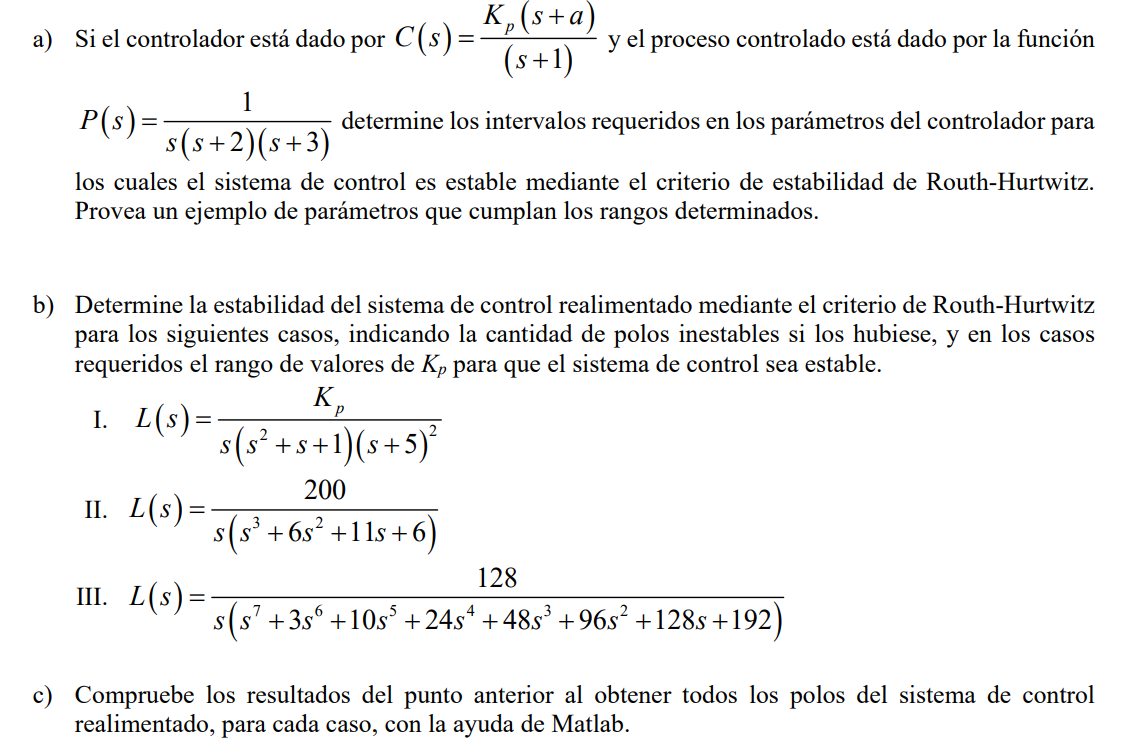
\includegraphics[width=\textwidth]{./tarea2/enunciado.png}
  \end{figure}
  \begin{enumerate}
    \item 
    Se obtiene el polinomio caracterítico del sistema.
    \begin{align*}
      1+C(s)P(s) &= 1+\frac{K_p(s+a)}{s(s+1)(s+2)(s+3)} = 0
      \\
      0 &= \frac{s(s+1)(s+2)(s+3)+K_p(s+a)}{s(s+1)(s+2)(s+3)}
      \\
      0 &= (s^2+s)(s^2+5s+6)+K_ps+K_pa
      \\
      0 &= s^4+5s^3+6s^2+s^3+5s^2+6s+K_ps+K_pa
      \\
      0 &= s^4+6s^3+11s^2+(6+K_p)s+K_pa
    \end{align*}

\renewcommand{\arraystretch}{1.5}
  \[
    \begin{matrix}
    \hline
    s^4 & 1 & 11 & K_p a
    \\\hline
    s^3 & 6 & 6+K_p & 0
    \\\hline
    s^2 & \frac{66-(6+K_p)}{6} & K_p a & 0
    \\
     & 66-6-K_p & 6K_p a & 0
    \\
     & 60-K_p & 6K_p a & 0
    \\\hline
    s^1 & \frac{(60-K_p)(6+kp)-36K_p a}{60-K_p} & 0 & 0 
    \\
     & 360+54K_p-K_p^2 - 36K_p a & 0 & 0
    \\
     & -K_p^2 + (54-36a)K_p + 360 & 0 & 0
    \\\hline
    s^0 & 6K_p a & 0 & 0
    \\
     & K_p a & 0 & 0
    \\\hline
    \end{matrix}
  \]

    \item hola 2

    \item hola 3
  \end{enumerate}
\end{ejercicio}